\chapter{Introduction}
This thesis compares methods from the field of artificial intelligence in their
ability to learn from reinforcement when trading electricity in simulated
competitive marketplaces.  An introduction to electric energy and the
associated markets is provided by the present chapter.  An explanation of the
motivation for the research presented in this thesis follows, along with a
statement of the principle contributions that have been made.  A outline of the
remaining chapters is finally provided.

\section{Electricity}
Electricity is a form of energy that has become the life-blood of modern
societies.  The popularity of electricity stems from the ease with which it may
be converted into light, heat and kinetic energy.  The average total demand for
electricity in the UK is now approximately 50GW.  The cost of buying 1MW of
electricity for one hour is around �40.  This equates to yearly transaction
values of \pounds17.52 billion.  The New York black-out in August 2003 involved
61.8GW of lost power supply to approximately 50 million consumers.  The majority
of supplies were restored within two days and the event is estimated to have
cost \$7-10 billion.

Quality of life for a person is directly proportional to that person's
electricity consumption[ref].  The world population is currently 6.7 billion
and forecast to pass 9 billion by the year 2050.  Electricity production
currently demands over $1/3$ of the annual primary energy extracted.  As people
endevour to improve their quality of life, primary energy fuels will become
increasingly scarce.  Competitive markets are a proven device for allocation
of scarce resources.

Commercialisation of electricity supply industries is a new practice, relative
to other commodities, having begun in the early 1990s.  The inability to store
electricity, once generated, in a commercially viable quantity prevents trade
as a conventional commodity.  Trading mechanisms must be created to allow
shortfalls in electric energy to be purchased a short notice from quickly
dispatchable generators.  Different implementations have been tried in various
countires and states and how best to structure electricity markets is an open
field of research.  Electricity market designs are further complicated by the
need to manage complex dynamic constraints in the power systems that deliver
the traded product.

\section{Electricity Markets}
% The Electric Lighting Act 1882 began the development of the UK's electricity
% supply industry by allowing persons, companies and local authorities to set up
% supply systems\cite{wikipedia:timeline}, principally at the time for the purposes
% of street lighting and trams\cite{eyles:bath}.  Under The Electricity Supply Act
% 1926 the Central Electricity Board started operating the first grid of regional
% networks interconnected and synchronised at 132kV, 50Hz in 1933.  This began
% operation as a national system five years later in 1938 and was nationalised
% under The Electricity Act 1947 with the merger of over 600 electricity companies
% and the creation of the British Electricity Authority.  This was then dissolved
% and replaced with the Central Electricity Generating Board (CEGB) and the
% Electricity Council under The Electricity Act 1957.  The CEGB was responsible for
% planning the network and generating sufficient electricity until the start of
% privatisation in 1990 when it was split into The National Grid Company and three
% generating companies: Powergen (now owned by German Utility E.ON), National Power
% and Nuclear Electric (Nuclear Electric + Scottish Nuclear = British Energy).  The
% Electricity Council set the prices for electricity according to financial targets
% set by the government.
%
% \subsection{The Electricity Pool}
% The privatisation of the UK electricity supply industry under Margaret Thatcher
% saw the creation of The Electricity Pool in March 1990 for the trading of
% electricity.  The control of the transmission system was transferred to The
% National Grid Company which is now publically listed, but was originally owned by
% twelve regional electricity companies.  The Pool was managed by the Pool
% Executive Committee (PEC) and was essentially a multilateral contractual
% arrangement between generators and suppliers, known as the Pool Settlement
% Agreement (PSA), and did not itself buy or sell electricity.  Competition in
% generation was introduced gradually, by only entitling customers with
% consumption greater than or equal to 1MW to purchase electricity form any
% listed supplier.  This limit was then lowered in April of 1994 to included
% customers consuming 100kW or more and finally to include all customers in 1998.
%
% \subsubsection{Market Mechanism}
% \begin{figure}
% 	\centering
% 	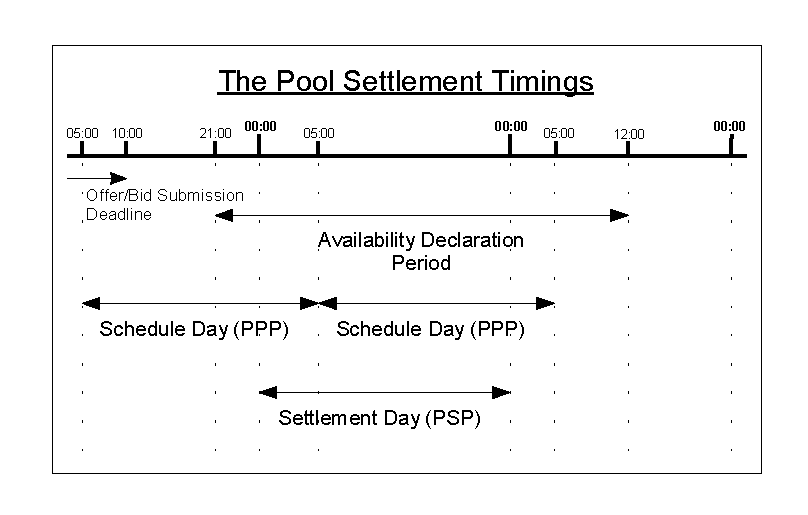
\includegraphics[width=11.7cm]{figures/settlement_times}
% 	\caption{England \& Wales Electricity Pool settlement timing
% 	diagram}%\cite{elecpool:about}}
% 	\label{fig:timing}
% \end{figure}
%
% The England \& Wales Pool mechanism enabled competition in both generation and
% retail supply, scheduling of generation was on a merit order basis at a day ahead
% stage and set a wholesale electricity price for each half-hour period of the
% schedule day.
%
% In The Pool forecasts, based on historic data and adjusted for factors such as
% the weather, of Total Demand in MW for each Settlement Period (every 30 minutes
% in this case) during the Availability Declaration Period (See Figure
% \ref{fig:timing}) were used by generating companies and organisations with
% interconnects to the England \& Wales grid such as Electricit\'e de France (EdF)
% and Scottish Power, to put together bids that must be submitted to the grid
% operator by 10:00 on the day before the Schedule Day.  These bids have a number
% of components which are explained in detail in section \ref{sec:offers}.  They
% are fed into a settlement computer program called GOAL (Generator Ordering and
% Loading) which calculates an Unconstrained Schedule, that is one which does not
% take into account the physical limitations of the transmission system, so as to
% meet the forecast demand and requirements for reserve while minimising cost.
% This is done using a merit order dispatch (cheapest bids up to the marginal point
% accepted first) and generally the bid price from the Marginal Generator is used
% to determine the System Marginal Price (SMP) for each Settlement Period.  The SMP
% is then used to determine the prices paid by consumers and paid to the generators
% (\S \ref{sec:prices}).  Variations in demand and changes in plant availability
% are adjusted for by the grid operator who may call on generators that submitted
% offers into the Pool or, more rarely, those that are contracted to provide
% ancillary services to increase or reduce production.  Alternatively, the grid
% operator may call upon large customers that have agreed to curtail their demand
% on request to do so.
%
% \subsubsection{Generator offer data}
% \label{sec:offers}
%
% \begin{figure}
% 	\centering
% 	
\includegraphics[width=11.7cm]{figures/pool_bid_chart}
% %	\caption{Diagram of the The Pools bid structure\cite{sweeting:pool}}
% 	\label{fig:poolbids}
% \end{figure}
%
% Bids submitted to The Pool consisted of five price parameters (See Figure
% \ref{fig:poolbids}) and represented the avoidable cost of generation
% \cite{sweeting:pool}.  The start-up price would represent the cost of starting
% the generator up from cold.  The no-load price would be the cost in pounds of
% keeping the generator running, regardless of its output and the three incremental
% prices specify the cost per MWh of generation at different levels.  Bids
% including this information would be submitted for each half hour settlement
% period and any bids that do not conform to the standard or are not submitted are
% substituted with values from the last valid declaration.
%
% \subsubsection{Price determination}
% \label{sec:prices}
%
% Essentially, the bid from the marginal generator in the unconstrained schedule
% would set the System Marginal Price (SMP) for a specific Settlement Period.
% However, the prices paid by the consumers, the Pool Selling Price (PSP), and the
% prices paid to the generators, the Pool Purchase Price (PPP) would be adjusted in
% order that the costs of transmission be covered by the market and that the
% availability of capacity be encouraged at certain times.
%
% The PPP is made equal to the System Marginal Price plus a capacity payment, which
% is generally the Loss of Load Probability (LOLP) multiplied by the Value Of Loss
% of Load (VOLL) minus the SMP.
%
% \begin{equation}
% PPP = SMP + LOLP(VOLL-SMP)
% \end{equation}
%
% The LOLP is an estimate of the probability that, due to a lack of spare
% generation capacity, the system would fail and the VOLL is an estimate of the
% financial loss that a customer would incur if supply was not possible.  This PPP
% is the payment received by generators that were included in the original
% unconstrained schedule and were called on to supply.
%
% \begin{table}
% \doublespacing
% 	\centering
% 	\begin{tiny}
% 	\begin{tabular}{|c|c|c|c|}
% 	\hline
% 	& & \multicolumn{2}{|c|}{Actual Schedule} \\
% 	\hline
% 	 & & In & Out \\
% 	\hline
% 	\multirow{2}{2cm}{Unconstrained Schedule} & In & $SMP + LOLP(VOLL - SMP)$ & $SMP - BID + LOLP(VOLL-SMP)$ \\
% 	 & Out & $BID + LOLP(VOLL - BID)$ & $LOLP(VOLL - BID)$ \\
% 	\hline
% 	\end{tabular}
% 	\end{tiny}
% %	\caption{Payments to generators under The Pool\cite{ofgem:1998}}
% 	\label{tab:payments}
% \singlespacing
% \end{table}
%
% Table \ref{tab:payments} shows the payments made to generators under other
% circumstances.  Generators included in the unconstrained schedule but, due to
% perhaps lower demand than forecast or constraints from the transmission system,
% did not supply are paid the same minus their bid price.
%
% Generators may also receive payment for the provision of ancillary services
% according to their contract with the grid operator\cite{sweeting:pool}.



\section{Problem Statement}%/Aims \& Objectives}
% Free market democracy has underpinned the transformation of large western
% economies in the post war era and continues to be relied upon.  Towards the
% end of the nineteenth century the principals of competitive trade were
% successfully applied to electric power industries, beginning in the UK in March
% 1990 with the creation of The Electricity Pool.

% Two trends characterise modern power systems Engineering:
% Increased liberalisation of the industry through competitive energy trade and
% increased presence of renewable energy generation on the network.  As the
% number and variety of electricity sources becomes greater, the necessity for
% automated trade of their power increases.  Control algorithms may draw sensor
% input from data networks and other sources and use some relevant measure of
% performance, such as profitability, to learn from trading decisions.

% \IEEEPARstart{E}{nergy} consumers will often not switch suppliers despite
% apparent benefits of doing so, or mistakenly switch to more expensive
% contracts[].  Energy companies are thus unlikely to reduce prices as this
% can not be expected to result in new contracts.  One possible solution to this
% problem is to give the responsibility for buying energy to autonomous,
% learning control algorithms.  Drawing information from the internet and using
% standardised messaging [CIM] to form contracts, energy bots have the potential
% to introduce greater liquidity to energy markets and promote reduction of
% costs to the consumer.

Methods including learning classifier systems, genetic algorithms and
reinforcement learning have been successfully used to research the
charateristics of energy markets in the past\cite{anke:2008}.  This an
alternative to the traditional closed-form equilibrium approaches to game
theory research in which behavior emerges from the interactions of many
separable, self-serving agents. Typically in these studies, an agent is
associated with a portfolio of generating units and/or dispatchable
loads. Interaction with the environment involves submission of offers to sell
or bids to buy\footnote{Beware that certain authors may use the term ``bid''
to refer to an offer to sell when discussing single-sided auctions.} a
quantity of power at a specified price in a particular time period.  The
learning algorithms typically use revenue or earnings as a reward signal and
adjust the policy used to select offer/bid price and quantity values.

Research into energy trade using reinforcement learning typically
involves discretization the action domain, often into incremental markups
on marginal cost \cite{anke:2008}. Also, either sensor domains are discretized
or state information is disregarded altogether.  Despite these simplifications,
authors have been drawn many practical conclusions from this approach[ref].

In the field of robotic control, environment state, action and observation
spaces are often continuous or mixed.
% Learning methods using function approximation techniques such as connectionist
% systems have been developed for operation in such domains[ref].
Traditional reinforcement learning algorithms such as Sarsa and Q-learning can
be applied to systems with continuous domains by using connectionist systems
for value function approximation\cite{barto:neuron}. However, feedback
between policy updates and value function changes can result in oscillations
or divergence in these algorithms even when applied to simple
systems\cite{peters:enac}.  In response to this, policy-gradient methods,
pioneered by Williams\cite{williams:reinforce}, which search directly in the
policy space have been developed and applied in many real-life
settings\cite{barto:policy,shaal:robots,moody:direct,peshkin:routing}.

% \IEEEPARstart{D}{ynamic} competitive markets will be key in the transition
% to a low carbon economy\cite{decc:transition}.  Fluctuations in global oil
% prices have recently raised questions over the functioning of the energy
% market.  Energy industries in the UK contribute 4.8\% of 2.13
% trillion dollar gross domestic product.  The UK electricity industry supplies
% \~26 million customers with \~350TWh of energy each year at a cost of 3.5--9.0
% p/kWh. The New York blackout in August, 2003 resulted in the loss of 61.8
% GW of electric load associated with 50 million consumers.  Supply by was
% largely restored within two days and the event is estimated to have cost
% \$7--\$10 billion.  Small improvements in the design of markets associated with
% this industry can have an impact greatly upon the welfare of society and
% conversely also. To understand the complex dynamics of these systems it is
% possible to simulate them computationally.  One alternative to the game
% theoretic models typically employed in computational economics is the study
% of emergent behaviour in collections of individual autonomous actors.
%
% Representing competitive behaviour is key to the simulation of markets in this
% way. Simple heurisitc approaches have been taken in the study of
% \ldots[ConzelmannEMCAS].  While more complex machine learning techniques such
% as state vector machines have been employed in the study of market efficiency
% and market power[Bunn, Bagnall].  Reinforcement Learning (RL) is an
% unsupervised machine learning technique, most commonly applied to control
% problems, and as such is well suited to this
% application [Acrobot]\cite{suttonbarto:reinforcement}. [TD()]. In this paper
% RL is used to control the output and price of generating units and
% despatchable loads connected in a balanced three-phase high-voltage power
% system. RL has been applied before in a very similar manner to the energy
% trading problem using the Roth-Erev algorithm[TesfatsoRE].  The software
% implementation for this algorithm used in the simulations for this paper was
% translated from[TesfatsoAMES].

% Game theoretic models are commonly associated with economics and attempt to
% capture behaviour in strategic situations mathematically.  They have been
% applied to electric energy problems of many forms, including but not limited to
% analysis of market structure, market liquidity, pricing methodologies,
% regulatory structure, plant positioning and network congestion.  More recently,
% agent-based simulation has received a certain degree of attention from
% researchers and has been applied in some of these fields.
% \begin{quotation}
%  ``Every scientist knows the rule called Occam's Razor:  Faced with several
%  competing hypotheses, prefer the simplest one.  There is also an unspoken
%  corollary that might be called Occam's Castle:  Faced with several competing
%  places to build a new science, prefer the simplest one\ldots  Where the
%  foundation is firmest, the castle will rise highest.  Where the ground is
%  solid, build there, and the universe is so constructed that you will have a
%  view.''\cite{weiner:tlm}
% \end{quotation}

Engineers must strive for complexity in their work.  Rarely will a simple
solution will perform a function to a higher degree than a more complex one.
Certainly, where a function is either performed or not performed, prefer the
simpler one, but most often problems can be solved to varying degrees.

The broad aim of the research presented in this thesis is to prove that the
above conjecture applies to reinforcement learning algorithms for power trade.
Previous research in this field (See Chapter~\ref{ch:related_work} below) has
used very simple algorithms in relation to those from the latest advances in
artificial intelligence (See Sections~\ref{sec:enac}~and~\ref{sec:reinforce}
below).  The goal is to prove that policy gradient methods, using artificial
neural networks for policy function approximation, are better suited to
learning the complex dynamics of a power system.

\section{Research Contributions}
% The research presented in this thesis pertains to the academic fields of power
% engineering, artificial intelligence and economics.  The principle
% contributions in these areas are
%
% \begin{itemize}
%   \item The proof that policy gradient reinforcement learning algorithms
%   outperform value-function algorithms when applied to the power trade problem,
%   \item A novel coupling of power system models and optimal power flow
%   algorithm results with agents capable of handling discrete and continuous
%   sensor and action spaces,
%   \item Implementations of Roth-Erev reinforcement learning algorithms and
%   continuous versions of Q-learning and Q($\lambda$) for the open source
%   PyBrain library,
%   \item Open source implementations of power flow and optimal power flow
%   algorithms in the Python programming language, preserving sparsity throughout
%   the optimisation using the open source CVXOPT library.
% \end{itemize}
This paper compares policy-gradient reinforcement learning algorithms
REINFORCE and ENAC with value-function methods Roth-Erev, Q($\lambda$) and
Sarsa in their relative ability to trade electricity competitively.  Power
systems are modelled as balanced three-phase AC networks in the steady-state.
Offers/bids for active and reactive power from agent participants are cleared
using AC optimal power flow with an auction interface that returns single
period revenue and earnings values. Through individual and multi-player
experiments the methods are compared in their ability to learn quickly, compete
in large systems and exploit characteristics of the power system. It is shown
that, in electricity trade, policy-gradient methods:
\begin{itemize}
  \item converge successfully on an optimal policy,
  \item are slower to converge than value-function algorithms,
  \item can learn more complicated characteristics of the power system than
  value-function algorithms,
  \item scale better when applied to larger systems and reactive power markets.
\end{itemize}
Section~\ref{sec:opf} of this paper presents the power system model, the
optimal power flow formulation and the auction interface from MATPOWER.
Reinforcement learning methods Sarsa, Q($\lambda$), Roth-Erev, REINFORCE and
ENAC are defined in Section~\ref{sec:rl}. Section~\ref{ch:method} introduces
the three experiments used to compare the aforementioned methods. Numerical
results from these experiments are reported in Section \ref{ch:results} and
an interpretation and critical analysis of them is given in
Section~\ref{sec:discuss}.  Finally, a review of related research is presented
in Section~\ref{sec:related} and Section~\ref{ch:conclusion} provides a
conclusion.

\section{Outline}%Thesis structure/Overview/Reading guide}
This thesis is focussed on the application of standard and advanced
reinforcement learning algorithms to a particular problem domain.  The reader
will require a certain degree of prior knowledge, or must be willing to read
much of the referenced material, to fully understand the methodology taken.
The intended audience is engineering and economics researchers interested in
the application of reinforcement learning algorithms to the problem of trading
energy in electric power systems.

% Industrialised societies have become increasingly reliant on the supply of
% electric energy since the connection of large power stations began in 1938.
% The extent to which this is true can be seen in the financial impact that loss
% of supply has on society.
%
%
% In June 2004 the United Kingdom (UK) became a net importer of natural gas for
% the first time in 8 years[EIA DOE].  Since energy industry privatisation by
% the Conservatives in the 1980s, use of domestic gas reserves for electricity
% generation has been encouraged and exploited.
%
% % Insert dash for gas pie-chart here.
%
% As UK natural gas production has now peaked and consumption continues to grow,
% concern over reliance on imports from less stable regions has increased.
%
% The UK is hugely reliant on fossil fuels.  More than three quarters of UK
% electricity is generated from a relatively small number of large coal and gas
% fired power stations[Energy Digest].  Of the 298 stations with capacity over
% 1MW in the UK, 63 gas fuelled (including CCGT) and 13 coal fired stations
% supply over 290 TWh of the UK's 393TWh annual electric energy
% production[DUKES].  Much of the remainder is generated through nuclear
% fission.
%
%
% Concerns over climate change and security of supply have caused the UK
% government to pursue self-sustainable sources of electric energy.  This is
% illustrated by the government?s recent decision to make a legally binding
% commitment to an 80\% reduction in carbon dioxide emissions by 2050, relative
% to 1990 levels[].
%
%
% Relative to most other commodities, trade of electric energy is still in its
% infancy.  Liberalisation and unbundling of electricity supply industries costs
% many millions of pounds to implement[].  Countries, having made this
% investment, continue to restructure and adjust their energy markets in the
% hope of further reducing costs to the consumer and promoting innovation and
% efficiency through competition.
%
%
% \section{Conventional national power systems}
% Economies of scale prompted construction of the first large-scale power
% stations in the UK at the beginning of the twentieth century.  Following the
% introduction of the Electricity (Supply) Act 1926 the largest and most
% efficient of these were connected by a series of regional high-voltage
% three-phase AC grids synchronised at 50 Hertz.  Integration was completed and
% a national transmission system made operational in the UK for the first time
% in 1938.  This approach to electricity supply is largely the same as that
% still employed throughout the UK to the present day.  Alternating current,
% mainly from rotating synchronous machines, is transformed to high voltages for
% bulk transmission over long distances with high efficiency.  Power from the
% transmission system is fed through distribution networks in a uni-directional
% fashion at lower voltages before final usage.
%
% While maintenance and extension of the transmission system and of distribution
% networks is an everyday activity for energy utilities, many power system
% components have extremely long operational lifetimes[].  This and the
% magnitude of the capital investment made post-war in construction of the
% electricity networks suggests that there is likely to be little change in the
% topology of the system of wires in the foreseeable future.  This is further
% compounded by the fact that distribution networks are often radial in their
% structure.  Reliability and protection are major issues in the operation of
% power systems and the task of detecting and isolating a fault is often more
% difficult in systems that are meshed.
%
% Large-scale thermal power stations operate steam and gas turbines around 13
% metres in length, approximately 400 tons in weight and rotate at up to 3600
% revolutions per minute[SIEMENS].  The kinetic energy stored in these turbines
% and the connected synchronous machines is vast and the associated flywheel
% effect plays an important role in smoothing short-term imbalances in supply
% and demand[].
%
% Synchronous machines used in large thermal power stations invariably use a
% rotor winding that is excited and a magnetic flux created by a DC current.
% Controlling the magnitude of the rotor field current allows the reactive power
% provided or absorbed by the machine to be adjusted.  Reactive power is
% essential in maintaining system voltage within permissable limits[].
%
% \section{Highly distributed national power systems}
% The highly distributed power system is a conceptual future for the UK's
% national energy network.  It is capable of meeting current targets for reduced
% greenhouse gas emissions[] and reduces reliance on foreign fuel imports.  It
% is a system in which all but the least polluting fossil fuelled power stations
% have been decommissioned.  Their output supplanted by distributed generation,
% supported with demand-side management measures and advances in energy storage
% technology.
%
% Distributed (or embedded) generation is most easily defined as electricity
% production plant connected to the national electricity network at the
% distribution level[DG Book].  The transmission system being defined as that
% which operates at of above 275kV in England and Wales or at or above 132kV in
% Scotland.  This encompasses most small-scale plant, but there exist exceptions
% such as large-scale wind farms.
%
% Hydro-electric dams, biomass fuelled power stations and wind farms are the
% three sources of renewable energy currently available in the UK with
% capacities equivalent to that of fossil fuelled plant.  Hydro-electric power
% stations are often large-scale and transmission connected for bulk transport
% of power to load centres.  The low energy density of biomass fuels, relative
% to that of fossil fuels, often dictates that related generating plant is
% located close the fuel source origin and connected to a distribution network.
% The time varying nature of wind energy necessitates the use of induction
% machines for generation.  These are typically sinks of reactive power and
% require support for operation and maintenance of voltage.
%
% \subsection{Increased source granularity}
% In terms of demand the UK power system is already highly distributed.  The
% number of generators, controllable loads and storage systems is expected to be
% much greater in a HDPS.  However, there are at present already around 260
% generators supplying energy to consumers and the mechanisms currently in place
% to facilitate the trade of their power may be adaptable.
%
% Consumers and owners of small-scale generation will continue to desire
% protection from the risks associated with the wholesale marketplace.  Today?s
% typical domestic and commercial supply contracts between consumers and energy
% retailers offer such protection.  As the penetration of DER grows the role of
% energy retailers offering aggregation services will likely grow as more plant
% owners come to desire representation in the marketplace.  While there are a
% great many ways in which this aggregation may be arranged it remains
% essentially a contractual arrangement. A much larger challenge lies in the
% operation and control of a system in which the state of plant is principally
% determined by a decentralised free market.  The network may be divided
% into ?cells? for the provision of a single point of control, but each cell may
% contain individual items of plant being aggregated by different companies.
% Controlling the DER, so as to adhere to system constraints, must be done in
% the most economically efficient, in the least environmentally damaging manner
% and according to contracted access arrangements.  Also, the details of any
% control measures undertaken must be fed back to the marketplace such that they
% may be taken into consideration during the settlement process.  This interface
% between the technical domain and the commercial mechanisms remains an open
% research topic.
%
% \subsection{Inversion of control}
% Consumers have grown accustomed to using power from the grid at will.  System
% loads are by and large passive and, with the exception of dual rate white
% metered loads, only the largest make adjustments to their consumption
% according to price signals or system conditions.  It is likely that the
% fluctuating nature of the power output from generators exploiting renewable
% energy sources will necessitate an increase in the adoption of active loads.
% As control shifts from being almost purely supply-side, an opportunity opens
% for the energy marketplace to offer appropriate consumer choice, not only in
% terms of cost, but Quality of Service (QoS) also. Advances in smart metering
% promise to support such a migration.
%
% \subsection{Reduced network reticulation}
% The connection of controllable energy resources to lower voltage and less
% reticulated areas of the network may also offer new possibilities for
% structuring the relationship between the market and the system for management
% of network constraints.  There are generally three options for power system
% constraint management.
%
% \begin{itemize}
%   \item Only permit the formation of energy trades if delivery is physically
%   feasible.
%   \item Impose delivery charges which increase as network constraints are
%    approached.
%   \item Request extended bids and offers which include costs associated with
%   the adjustment of participant?s desired position.
% \end{itemize}
%
% The third option most closely describes the method currently used in the United
% Kingdom.  In a highly reticulated network it is difficult to determine the
% direction of each participant?s energy flows.  In turn, this poses
% difficulties in determining if a particular delivery is feasible and which
% participants are responsible for congesting the network.  Distribution
% networks are typically less reticulated than the transmission network to which
% the majority of generation is connected at present.  Therefore, there may be
% opportunities to utilise options one or two in an energy marketplace for an
% HDPS.
%
% Furthermore, the lower voltage of distribution networks may open up
% opportunities for more widespread use of power electronics technologies such
% as FACTS and phase shifting devices.  These would provide a limited ability to
% direct the flow of electrical energy.  How this might be managed on a wide
% scale and how efficient interaction with the marketplace might be achieved is
% open to investigation
%
% \subsection{Dual objective optimisation}
% Along with concern over the UK's dependence on natural gas imports, concern
% over the environmental impact of electricity generation is a primary motivator
% for a move to HDPS.  The energy market is expected to simultaneously minimise
% costs to the consumer and encourage reduced emission of greenhouse gasses.
%
% The European Union Greenhouse Gas Emission Trading Scheme (EU ETS) is an
% example of how a second marketplace running parallel to electricity trade, in
% this case trading allowances, may give weight to this new objective.  There
% are other ways in which the greenhouse gas output of certain technologies may
% be taken into consideration and this remains an open and important research
% topic.
